\documentclass[11pt, oneside]{amsart}

\usepackage{amsmath}
\usepackage{amssymb}

%\usepackage{multibbl}
%\usepackage{bibtopic}

\usepackage{color}
\usepackage{dcolumn}
\usepackage{float}
\usepackage{graphicx}
%\usepackage{graphics}
\usepackage[latin9]{inputenc}
\usepackage{multirow}
\usepackage{rotating}
\usepackage{subfigure}
\usepackage{psfrag}
\usepackage{tabularx}
\usepackage[hyphens]{url}
\usepackage{wrapfig}
\usepackage{framed,color}
\usepackage{fancybox}

%\setcounter{secnumdepth}{3}
%\setcounter{tocdepth}{3}


\usepackage[bookmarks, bookmarksopen, bookmarksnumbered]{hyperref}
\usepackage[all]{hypcap}
\urlstyle{rm}

\definecolor{orange}{rgb}{1.0,0.3,0.0}
\definecolor{violet}{rgb}{0.75,0,1}
\definecolor{darkgreen}{rgb}{0,0.6,0}
\definecolor{cyan}{rgb}{0.2,0.7,0.7}
\definecolor{blueish}{rgb}{0.2,0.2,0.8}

\definecolor{shadecolor}{rgb}{0.9,0.9,0.9}

\newcommand{\todo}[1]{{\color{blue}$\blacksquare$~\textsf{[TODO: #1]}}}
\newcommand{\huttonnote}[1]{ {\textcolor{magenta}    { ***Eric:      #1 }}}
\DeclareRobustCommand{\csdms}{\textsc{csdms}}

% Don't use tt font for urls
\urlstyle{rm}

\begin{document}

\title[]{Building Sustainable Software - The CSDMS-2.0 Approach}

\author{
  Eric W. H. Hutton$^{\dag}$,
  Mark D. Piper$^{\dag}$,
  Irina Overeem$^{\dag}$
  Albert J. Kettner$^{\dag}$,
}

\thanks{{}$^{\dag}$ Community Surface Dynamics Modeling System, Boulder, CO}

\begin{abstract}

The Community Surface Dynamics Modeling System (\csdms{}) is an NSF funded
project whose focus is to aid a diverse community of earth and ocean system
model \emph{users} and \emph{developers} to use and create robust software
quickly.  To this end, \csdms{} develops, integrates, archives and disseminates
earth-system models and tools to an international (67 country) community
with the goal of building a complete set of tools necessary to model the
earth system. \csdms is a place modelers look to for access to hundreds open
source surface-dynamics models and tools, as well as model metadata. Such a
model repository increases model transparency and helps to eliminate the
duplication of effors by presenting the current state of modeling efforts.
To increase software sustainability, composability and interoperability \csdms
promotes standards that define common modeling interfaces, semantic mediation
between models, and model metadata. Through online resources and workshops,
\csdms promotes software engineering best practices, which are foreign to many
developers within our modeling community. For example, version control, unit
testing, continious integration, test-driven development, well-written
\emph{clean code}.

\end{abstract}

\maketitle

\section{The Community Surface Dynamics Modeling System}

The Community Surface Dynamics Modeling System (\csdms{})
~\cite{peckham2012component}
is an NSF-funded project that began in 2007. Its mission is to help a diverse
community of surface dynamics model \emph{developers} and model \emph{users}
work together toward
common goals and standards. Part of this effort involves creating a repository
of open-source models. Another part involves converting models to plug-and-play
components that can be reused via dynamic linking within the \csdms framework to
create new models. In building its modeling framework, \csdms has leveraged
several existing, well-established and open-source software tools. For example,
\csdms uses three tools from the Common Component Architecture (CCA) toolchain:
Babel, Bocca and Ccaffeine. Babel provides interoperability between components
written in different languages; it currently supports C, C++, Fortran, Java,
and Python. Bocca helps with creating CCA-compliant components and managing CCA
component projects. Ccaffeine is a CCA-compliant framework for linking
components into new applications. All three tools were designed to enable
component-based modeling in an HPC environment, but they can also be used on
desktop systems. \csdms has developed innovative model/component interfaces for
use with the CCA tools, including the Basic Model Interface (BMI), which uses
the \csdms Standard Names (both described below) and the framework-level
Component Model Interface (CMI). \csdms has also developed a web-based client
for its modeling framework (the \csdms Web Modeling Tool, WMT, described below)
that allows users to compose new models by connecting and configuring
components through a simple, browser-based graphical interface.

In order to realize the full power and benefits of component-based modeling, a
modeling framework like \csdms needs an efficient mechanism to convert as many
open-source models as possible to reusable plug-and-play components. Since this
necessarily requires some involvement from each model's developer, this
mechanism must be designed to:

\begin{itemize}

\item require minimal effort from the model developer,

\item allow the model to continue to be used in a stand-alone manner,

\item not introduce new dependencies into the model,

\item not interfere with the developer's design,

\item not require any modeling framework-specific knowledge on the part of the
      developer,

\item not require the addition of new code which accommodates the needs of
      other models. 

\end{itemize}

These requirements became clear during the first few years of the \csdms project
by working directly with model developers and listening to their concerns and
complaints about early designs and other frameworks.

\section{Building a User Community}

\csdms{} provides cyber-infrastructure to promote the quantitative modeling of
earth surface processes. The US National Science Foundation funds CSDMS, but
the community is international and includes industry and federal agency
representatives in addition to members from academic institutions. The
initiative has been growing with >150 people per year. CSDMS now fosters a
community of ~1150 scientists who work on prediction of the movement of fluids,
and the production, erosion, transport, and deposition of sediment and
nutrients in landscapes and seascapes. 

\section{Model Repository}

Software accessibility is a key value of the CSDMS mission. CSDMS ensures that code developed by individual researchers or small research teams remains accessible beyond the lifetime of a specific research project. Code developers are coaxed into providing their codes under open-source licenses. 

CSDMS has built an online model repository that importantly documents the submitted code with metadata, smoke-tests codes on the CSDMS High Performance Computing Cluster, maintains a snapshot of submitted source code in a version-control system, and provides easy downloads of the original source code. This repository now contains 172 codes and 56 tools, or 4,074,236 lines of source code (a source code line is defined as any line that is not part of a comment, and is not blank).

We do know our community values this resource, we track downloads of each individual code and the total number of downloads since November 2008 is >13,218 (as of July 2014).

\section{Software sustainability through expanded functionality}

Another important goal of CSDMS is to enable the rapid development and application of linked dynamical models tailored to specific landscape-basin evolution problems and at specific temporal and spatial scales. Interdisciplinarity and coupling is a critical step towards advancing predictive modeling~\cite{voinov2010community}.

CSDMS develops a modeling environment containing a suite of integrated, ever-improving software modules, with expanded functionality beyond the original stand-alone codes. 

The modeling coupling framework is designed to catalyze Earth-surface process research by empowering a broad community of scientists, students and applied modelers with computing tools, streamlining the process of idea generation and hypothesis testing through linked surface dynamics models, and enabling rapid creation and coupling of models tailored to specific settings, scientific problems, and time scales

\section{CSDMS has an educational mission}

WMT provides the ability to run models with an easy to use graphical interface and intends to serve novice and more experienced modelers alike. The WMT beta version was released in May 2014  as a sequel to the CMT.   IF staff habitually evaluates the effectiveness of this tool and uses the feedback to improve the functionality: modeling courses at the University of Colorado, clinics at the International Summer Institute at the University of Minnesota, and clinics at annual CSDMS Annual Meetings are the dominant forums for this testing. 

Over the last 4 years >150 graduate students were enrolled in intensive modeling courses, originating from geography, hydrology, geology, oceanography, earth sciences and engineering departments. These courses provided an excellent use case for us to test usability and access to the tool. Students reported in post-course surveys that they were unfamiliar with the use of models on a high performance computing cluster beforehand (rated their familiarity as 1.5 average on a scale of 1-5), but ended the courses with familiarity and being more comfortable with running and changing simulations as well as visualizing results (average rating approaches 4 on a Likert scale of 1-5). 

Focused hands-on clinics at meetings also allowed more than 150 CSDMS members to experience the ease of use of CMT, and now WMT, and try several examples of how to use the tool. 

Course and clinic materials are posted online as educational resources. IF staff are developing WMT-specific help pages for all models currently available as components, so that users can easily learn about model parameters and input files. In addition, IF staff members are developing web-based video tutorials that show how to run models.

\section{The Basic Modeling Interface}

The \emph{Basic Modeling Interface} (BMI) is a component-coupling library
interface specification designed by \csdms~\cite{peckham2012component,
syvitski2014plug}.  In this context, a component is software that models a
particular environmental process and can be "plugged into" another component.

The BMI specification was designed without any particular model-coupling
framework in mind.  Rather, it was designed to be framework agnostic. We
recognize model-coupling frameworks and tools may come and go but the
functionality a framework requires from its components will be significantly
more long-lived. Thus, a component should outlive any framework that it might
operate within.

The BMI identifies the entry points into software components that provides a
calling appication with the necessary level of control to connect components.
\csdms, as well as other modeling frameworks such as
ESMF~\cite{hill2004architecture}, OpenMI~\cite{gregersen2007openmi}, and
OMS~\cite{david2002object}, identifies an interface that, at a minimum,
provides functionality to \emph{initialize}, \emph{update}, and
\emph{finalize} a component. However, for more tight coupling the components
must implement an interface to provide data access, and model metadata.

\csdms has found that BMI is an acceptable target for model developers. The use
of BMI has also dramatically reduced the effort required by \csdms staff to
create and maintain components. So long as a model component strictly exposes
a BMI, it can automatically be incorporated into the \csdms model-coupling
framework where it can then connect to compatible components to form larger
models.

%The introduction of the
%\csdms Standard Names provides a practical and elegant solution to the semantic
%mediation problem and Babel solves the language interoperability problem.
%\csdms has also assembled a large repository of surface process models that now
%includes over 171 open-source models and 56 tools. The repository contains
%terrestrial, coastal, marine, hydrological, carbonate and atmospheric models.
%Geodynamic, atmospheric and ecosystem models will be added over the next few
%years.

%So far, 55 of the 171 models have been wrapped for use as reusable
%plug-and-play components (although only 6 are currently visible in the new WMT).


\section{CSDMS Standard Names}

\huttonnote{Taken from the SSI proposal. I need to rewrite this.}

The \csdms Standard Names are a lingua franca for variable names between model
components. They play an important role in the BMI as they provide a mapping of
a model's internal variable names to a common language used by the BMI getter
and setter functions.

Most models require input variables and produce output variables. In a
component-based modeling framework, like \csdms, a set of components becomes a
complete model when every component is able to obtain the input variables it
needs from another component. The \csdms Standard Names were developed to
provide a practical solution to this semantic mediation problem
~\cite{peckham2012component, syvitski2014plug}.
While the CF Convention Standard Names, which were
introduced in the domain of the ocean and atmosphere model domains, have
somewhat overlapping goals, the \csdms Standard Names provide a more
comprehensive set of naming rules and patterns for creating unique labels for
model variables that are not specific to any particular modeling domain.

%The \csdms Standard Names are currently being extended to solid Earth modeling
%domains, including geodynamics, seismology, electromagnetic induction and
%petrology, in the framework of the "Earth System Bridge" EarthCube project led
%by PI Peckham. They also serve as the base for the metadata standard for
%numerical models (MMF) which is currently in development within \csdms.

%We are acutely aware of multiple other efforts to provide cross-domain
%ontologies in the realm of geosciences. PIs Peckham and Kelbert are involved
%with the initial steps in semantic crosswalk development recently initialized
%within the EarthCube community that aim to achieve synergy between these
%currently divergent metadata ontologies.


\section{Reusable Components}


\subsection{The \csdms Modeling Framework}


\subsection{Connecting Components with the Web Modeling Tool}

\huttonnote{Taken from the SSI proposal. I need to rework this a bit.}

The \csdms Web Modeling Tool (WMT; https://csdms.colorado.edu/wmt) is the
web-based successor to the desktop Component Modeling Tool. WMT is a web
application that provides an Ajax client-side graphical interface (the WMT
client) and a RESTful server-side database and API (the WMT server) that allows
users to build and run coupled Earth system models on a high-performance
computing cluster (HPCC) from a web browser.
WMT was designed with four objectives:
\begin{itemize}

\item  \emph{Accessibility}. As a web-based application, if you have access
to the Internet, you have access to WMT.

\item  \emph{Integration}. Easily hyperlink from WMT to resources on the \csdms
portal - including model documentation, labs, lectures, tutorials and
movies - or to other resources on the Internet.

\item \emph{Portability}. WMT has a native JavaScript interface, so it can be
accessed on any modern web browser, including tablet and mobile
versions of browsers.

\item \emph{Maintenance}. Because modern browsers tend to adhere to web
standards, which lead to fewer cross-compatibility issues than
operating systems, only one version of WMT needs to be developed
and maintained.

\end{itemize}

With WMT, a user can:

\begin{itemize}

\item select a Common Component Architecture (CCA) component model
      from a list to run in standalone mode;

\item build a coupled model from multiple CCA components organized as nodes
      of a tree structure;

\item  view and edit the parameters of the model components;

\item save models to a server, where they can be accessed on any computer
      connected to the Internet;

\item share saved models with others in the community;

\item run a model by connecting to a remote HPCC where the components are
      installed.

\end{itemize}

Although WMT is web-based, the building and configuring of a model can be done
offline. Reconnection is necessary only when saving a model and submitting it
for a run.

\begin{figure}
  \caption{The \csdms Web Modeling Tool}
  \begin{center}
    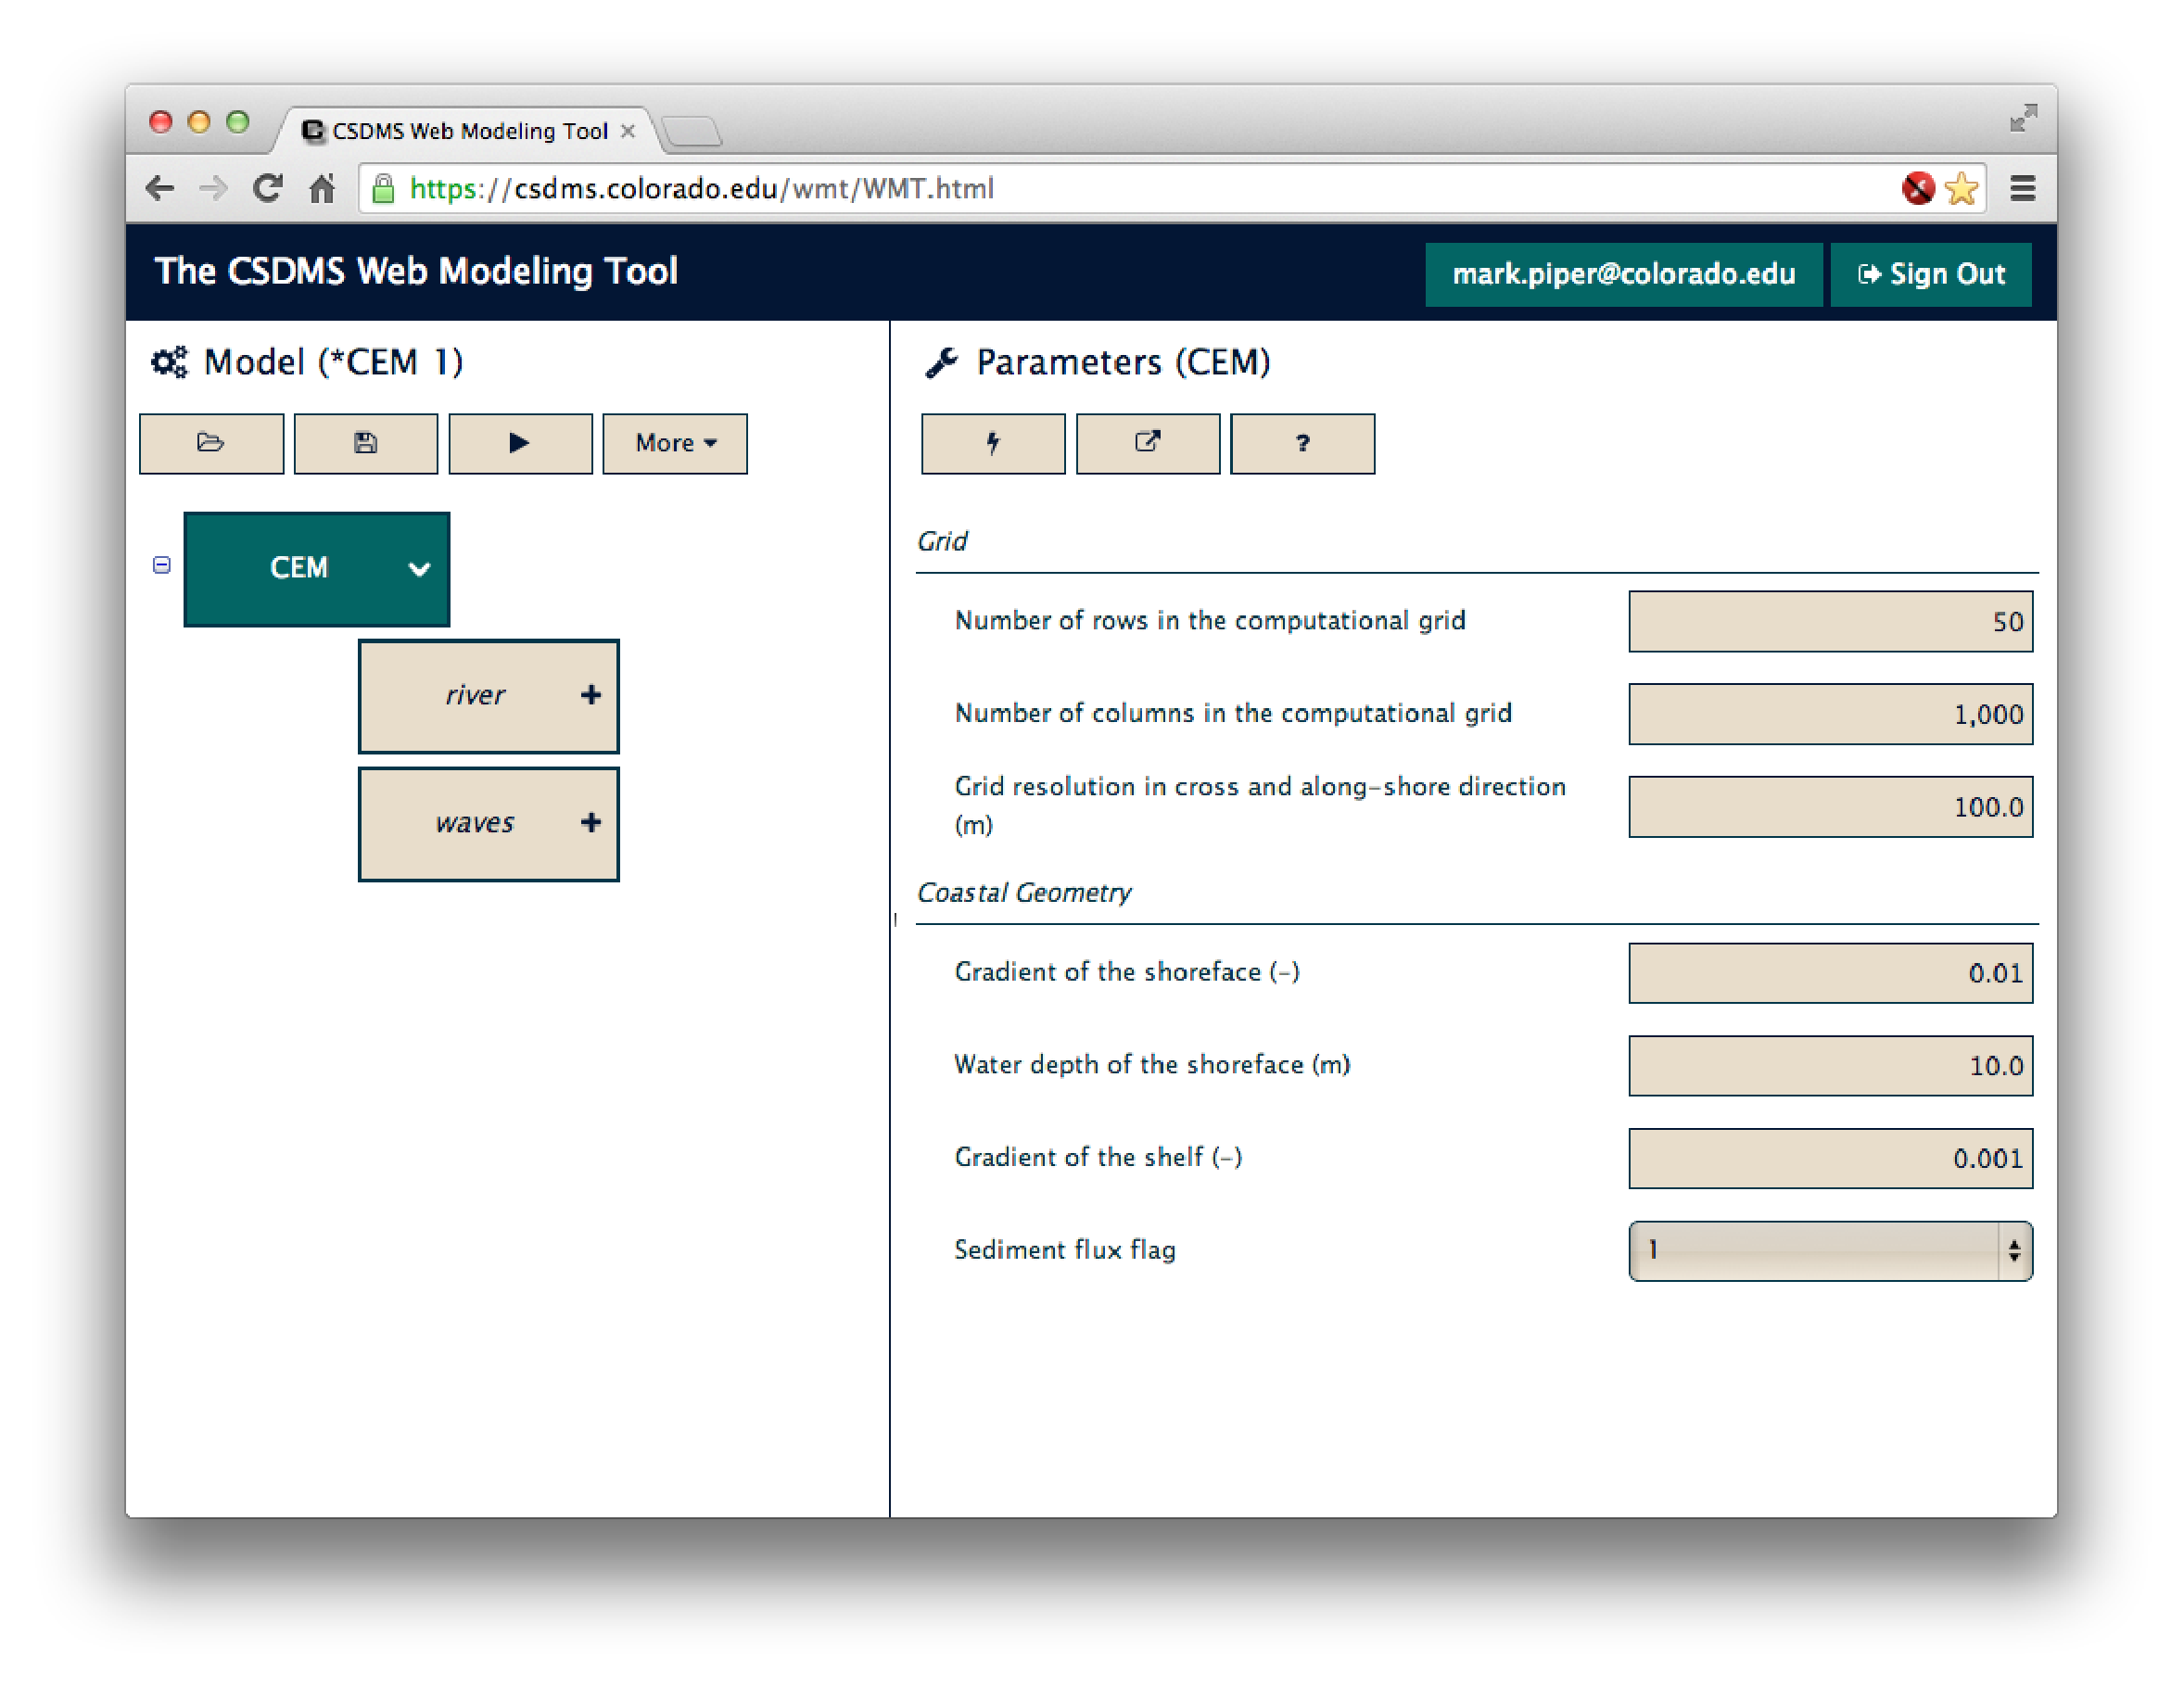
\includegraphics[scale=.25]{wmt.eps}
  \end{center}
  \label{fig:wmt_screenshot}
\end{figure}

\section{Digital Object Identifiers for Numerical Models}

\csdms is a strong advocate of truly open source software.  We believe this to
reduce redundancy, provide transparency through external review and make
research replicable, which is fundamental to scientific practices
~\cite{ince2012case}. \csdms acts as a venue through which open source code of
earth surface models are promoted, either by hosting or pointing towards open
source software. A Digital Object Identifier (DOI) system is implemented to
guarantee recognition to open source software contributors. DOI systems are
typically used to identify intellectual property in the digital environment.
It is used principally by publishers, and is an implementation of the Handle
System for persistent identifiers. The International DOI Federation (IDF)
appoints Registration Agencies who allocate DOI prefixes, register DOI Names,
and provide the necessary infrastructure to allow registrants to declare and
maintain metadata. \csdms is among the first software venues to assign DOIs to
open source software. The advantages of adopting a DOI system for open source
software are: 
\begin{itemize}
\item Guarantee credit to the software developer
\item Easily reuse and replicate research as software is directly locatable 
\item Increase software visibility, DOI content is 5 times more likely to
      deliver active links than content without.
\item Provide e.g. funding agencies the ability to track usage, so measure
      impact.
\end{itemize}

\csdms requests its DOIs through the Integrated Earth Data Applications (IEDA),
a formal Publication Agent of the DOI system that operates through the German
National Library of Science and Technology. Only stable versions of open source
software that are physically hosted through the \csdms repository will get a DOI
assigned. For model software citations, \csdms recommend following the DataCite
guidelines~\cite{brase2009datacite}. Interpreting these guidelines a citation
should have the following construction:

\begin{shaded}
\leftskip 0.25in
\parindent -0.25in
\tt{
Developer, A., Developer, B. (Year of publication). \emph{Name of the model},
Model Version. Identifier.
}
%\emph{ModelDeveloper(s)}, (\emph{PublicationYear}). \emph{ModelName},
%\emph{ModelVersion}. \emph{Identifier}.
\end{shaded}

The DOI system for numerical models is adopted by
\csdms as an incentive towards the earth surface processes community, to
stimulate contributions towards open source software by ensuring recognition
towards its developers.


\section{Acknowledgements}

The \csdms Integration Facility operates under continuing grant 0621695 from the
US National Science Foundation.

\bibliographystyle{plain}

\bibliography{wssspe-citations}{}

\huttonnote{Add something about model DOIs in the abstract}

\huttonnote{
\begin{itemize}
\item improving the development process that leads to new software
  \begin{itemize}
  \item methods to develop sustainable software from the outset
  \item effective approaches to reusable software created as a by-product of
        research
  \item impact of computer science research on the development of scientific software
  \end{itemize}
\end{itemize}
}

\huttonnote{This is Irina's section.}

\huttonnote{
\begin{itemize}
\item building large and engaged user communities
  \begin{itemize}
  \item developing strong advocates
  \item measurement of usage and impact
  \end{itemize}
\item encouraging industry's role in sustainability
  \begin{itemize}
  \item engagement of industry with volunteer communities
  \item incentives for industry
  \item incentives for community to contribute to industry-driven projects
  \end{itemize}
\item improving education and training
  \begin{itemize}
  \item best practices for providing graduate students and postdoctoral
        researchers in domain communities with sufficient training in
        software development
  \item novel uses of sustainable software in education (K-20)
  \item case studies from students on issues around software development in
        the undergraduate or graduate curricula
  \end{itemize}
\end{itemize}
}

\huttonnote{This is Albert's section (he's rewriting this)}

\huttonnote{
\begin{itemize}
\item recommending policy changes
  \begin{itemize}
  \item software credit, attribution, incentive, and reward
  \item issues related to multiple organizations and multiple countries, such
        as intellectual property, licensing, etc.
  \item mechanisms and venues for publishing software, and the role of
        publishers
  \end{itemize}
\end{itemize}
}


\end{document}
